\documentclass[Thesis.tex]{subfiles}
\begin{document}

\chapter{{\sc ConformalLab} - Conformal maps and uniformization}
\label{chp:conformallab}

\begin{figure}
\centering
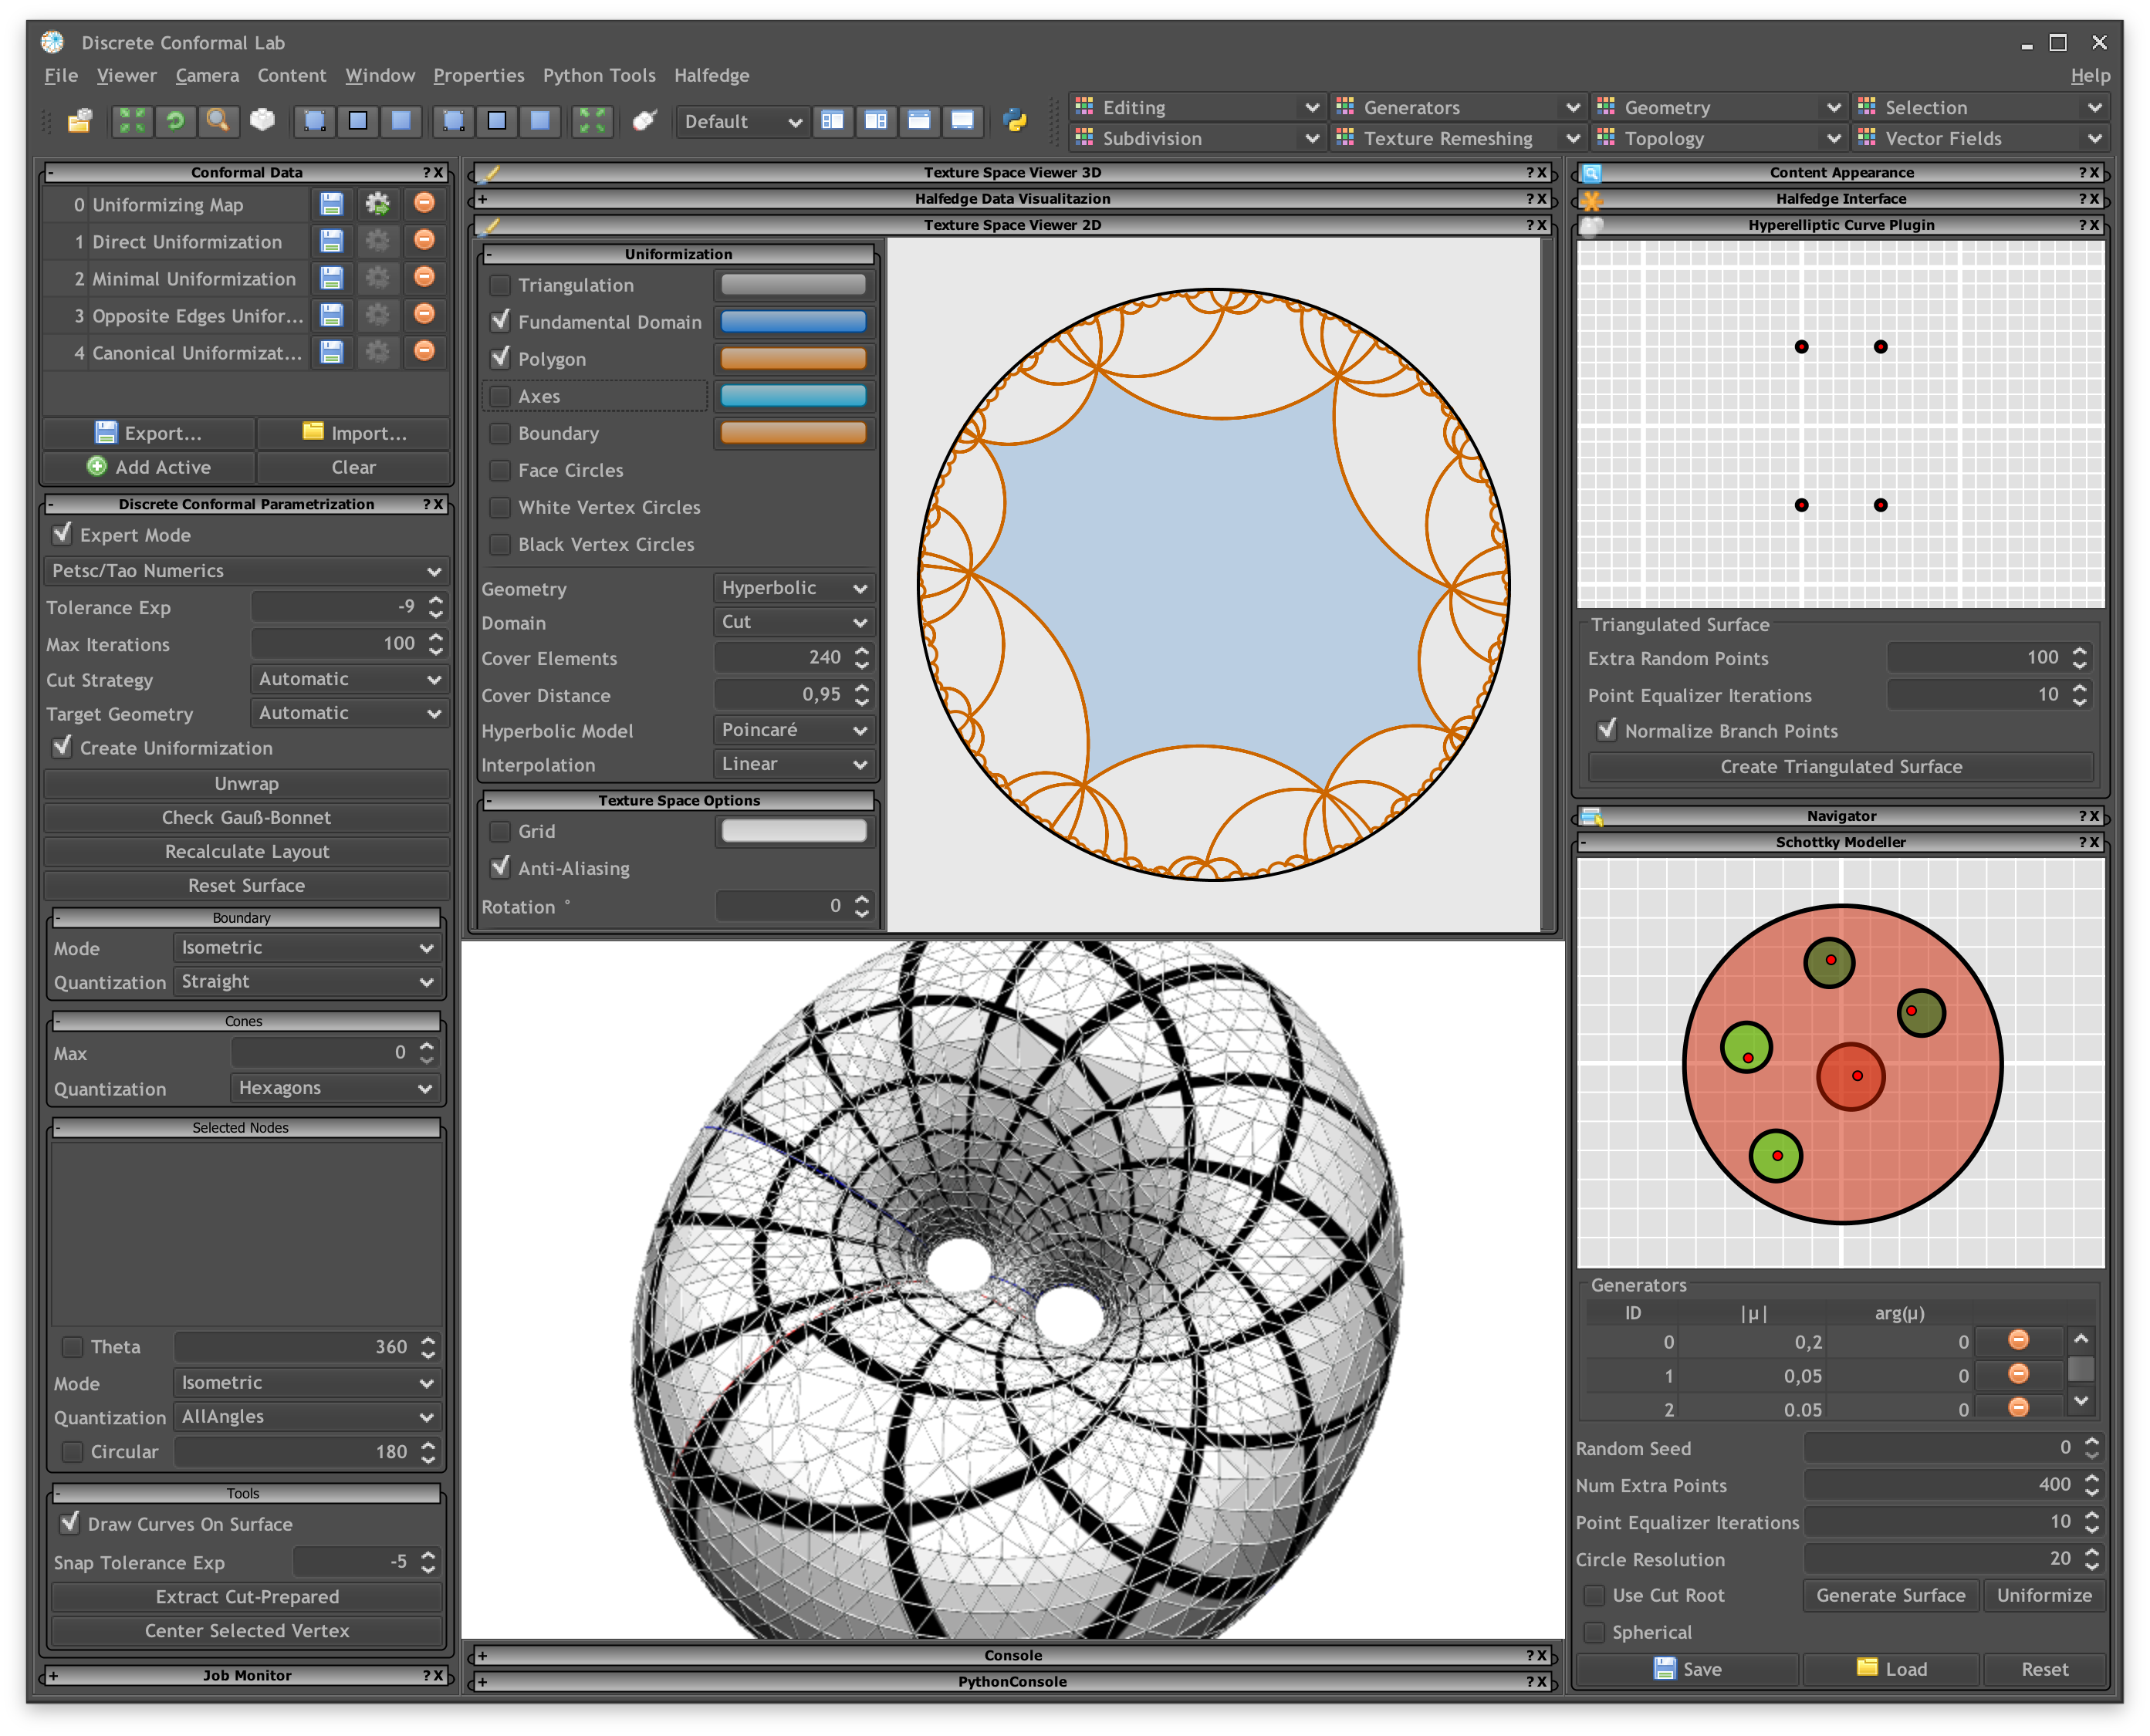
\includegraphics[width=0.7\linewidth]{conformllab/conformallab.png}
\caption{The window of {\sc ConformalLab}.}
\label{fig:conformal_window}
\end{figure}

This chapter enables the reader to reproduce examples contained in this work that involve uniformization of
Riemann surfaces, see Chapter~\ref{chp:conformal_examples}, and applications of conformal mappings of 
Part~\ref{part:applications}. The author has written {\sc Java} software, {\sc ConformalLab}, to calculate the corresponding data.
The software and the correponding data is included on the accompanying CD. 

{\sc ConformalLab} is designed to be used via a graphical user interface, see Figure~\ref{fig:conformal_window}. To store
resulting data an XML format is used. We describe this format in Section~\ref{sec:conformal_data}. The graphical user interface
is described in Section~\ref{sec:conformallab_ui}.


\section{Data format}
\label{sec:conformal_data}
To store and process data {\sc ConformalLab} uses an {\sc XML} data format.
All examples presented in Chapter~\ref{chp:conformal_examples} are stored
in this format. 
All XML data is contained in the XML namespace 
{\tt http://www.varylab.com/conformallab/types}.


{\bf Schottky data} 

A Riemann surface can be given by Schottky data, see Section~\ref{sec:schottky_examples}. An example is shown in Listing~\ref{lst:schottky_xml}. {\tt SchottkyData} can include one or more {\tt SchottkyGenerator}s. A {\tt SchottkyGenerator} defines fix points $A$ and $B$, the complex number $\mu$, and a {\tt Circle}. This circle is required to contain $A$ and must not contain $B$. If there are more that one generator, then the circles
an their images must not intersect.

\begin{lstlisting}[label=lst:schottky_xml, caption={A torus given by schotty data}, numbers=none, language=XML, captionpos=b]
<SchottkyData name="Schottky">
	<SchottkyGenerator>
		<A re="-1.0" im="0.0"/>
		<B re="1.0" im="0.0"/>
		<Mu re="0.25" im="0.0"/>
		<Circle radius="1.3">
			<Center re="-1.6" im="0.0"/>
		</Circle>
	</SchottkyGenerator>
</SchottkyData>
\end{lstlisting}

{\bf Hyperelliptic data} 

Hyperelliptic algebraic curves as used in the examples of Section~\ref{sec:examples_elliptic} and \ref{sec:examples_hyperelliptic} are given by the location of their branch points in the complex plane. All points must be distinct. Listing~\ref{lst:hyperelliptic_xml} shows the XML representation
of an elliptic algebraic curve defining a Riemann surface of genus~$1$.

\begin{lstlisting}[label=lst:hyperelliptic_xml, caption={A torus given as hyperelliptic data}, numbers=none, language=XML, captionpos=b]
<HyperEllipticAlgebraicCurve name="Curve g2">
	<BranchPoint re="-0.5" im="-1.0"/>
	<BranchPoint re="0.5" im="-1.0"/>
	<BranchPoint re="1.0" im="0.0"/>
	<BranchPoint re="-1.0" im="0.0"/>
</HyperEllipticAlgebraicCurve>
\end{lstlisting}

{\bf Discrete data} 

To specify discrete data we use the concept of half edge data structure, see also Chapter~\ref{chp:halfedge}. Listing~\ref{lst:halfedge_xml}
shows the structure of a {\tt HalfedgeEmbedding}. {\tt Vertices} are assigned coordinates in $\mathbb RP^3$ and their index. {\tt Halfedge}
nodes specify indices of incident faces, edges, and vertices as defined in Section~\ref{sec:halfedge}. In addition the data needed to specify 
the combinatorics of the half edge datastructure one can specify identifications of vertices and edges. An {\tt Identification} node contains
all vertices that are identified. Consider a parallelogram fundamental domain of a flat torus. In the parallelogram all four vertices are identified
to form the topological torus. Also the edges of the parallelogram are identified. An {\tt EdgeIdentification} node defines the four half edges
that belong to the pair of half edges on the torus.

\begin{lstlisting}[label=lst:halfedge_xml, caption={A torus given as {\tt HalfedegeEmbedding}
with identified edge pairs and vertices.}, numbers=none, language=XML, captionpos=b]
<HalfedgeEmbedding name="Uniformizing Map_domain">
	<Vertex x="0.0" y="0.0" z="0.0" w="1.0" index="0"/>
	<Vertex x="1.0" y="0.0" z="0.0" w="1.0" index="1"/>
	<Vertex x="1.0" y="1.0" z="0.0" w="1.0" index="2"/>
	<Vertex x="0.0" y="1.0" z="0.0" w="1.0" index="3"/>
	<Identification>
		<Vertex>0</Vertex>
		<Vertex>1</Vertex>
		<Vertex>2</Vertex>
		<Vertex>3</Vertex>
	</Identification>
	<Halfedge left="0" target="1" next="1" opposite="4" index="0"/>
	<Halfedge left="0" target="2" next="2" opposite="5" index="1"/>
	<Halfedge left="0" target="3" next="3" opposite="6" index="2"/>
	<Halfedge left="0" target="0" next="0" opposite="7" index="3"/>
	<Halfedge left="-1" target="0" next="7" opposite="0" index="4"/>
	<Halfedge left="-1" target="1" next="4" opposite="1" index="5"/>
	<Halfedge left="-1" target="2" next="5" opposite="2" index="6"/>
	<Halfedge left="-1" target="3" next="6" opposite="3" index="7"/>
	<EdgeIdentification edge1="0" edge2="4" edge3="2" edge4="6"/>
	<EdgeIdentification edge1="1" edge2="5" edge3="3" edge4="7"/>
	<Face index="0"/>
</HalfedgeEmbedding>
\end{lstlisting}

The {\tt HalfedgeEmbedding} data type can be used to define disceret maps between discrete embeddings. A discrete map consists of
a domain {\tt HalfedgeEmbedding} and the correponding image. Both nodes must define the same number of vertices. The map is defined
via vertex indices. A vertex $i$ from the domain is mapped to the vertex with index $i$ in the image data structure, see Listing~\ref{lst:halfedgemap_xml}.

\begin{lstlisting}[label=lst:halfedgemap_xml, caption={A discrete map is given by a pair of {\tt HalfedgeEmbedding}s, the {\tt Domain} and {\tt Image} of the map. Both are of type {\tt HalfedgeEmbedding}.}, numbers=none, language=XML, captionpos=b]
<HalfedgeMap name="Uniformizing Map">
	<Domain name="Uniformizing Map_domain">
		...
	</Domain>
	<Image name="Uniformizing Map_image">
		...
	</Image>
</HalfedgeMap>
\end{lstlisting}

A way of defining a discrete Riemann surface is to specify its discrete metric. A {\tt DiscreteMetric} defines non-oriented {\tt MetricEdges}
and their lengths. {\tt MetricTriangles} are glues along those edges. All triangles are oriented by the order of edges defined by attributes
{\tt edge1}, {\tt edge2}, and {\tt edge3} respectively. By that we can ony encode oriented discrete Riemann surfaces using a {\tt DiscreteMetric}.
A simple example featurering a Wente torus is shows in Listing~\ref{lst:discretemetric_xml}.

\begin{lstlisting}[label=lst:discretemetric_xml, caption={A wente torus given by a discrete metric. Vertices are given implictly
by following the order of triangle glueings.}, numbers=none, language=XML, captionpos=b]
<DiscreteMetric name="Wente Torus">
	<MetricEdge length="1.0" index="0"/>
	<MetricEdge length="1.0" index="1"/>
	<MetricEdge length="1.0" index="2"/>
	<MetricTriangle edge1="0" edge2="1" edge3="2"/>
	<MetricTriangle edge1="0" edge2="1" edge3="2"/>
</DiscreteMetric>
\end{lstlisting}

{\bf Uniformization data} 

\begin{lstlisting}[label=lst:hyperelliptic_xml, caption={A torus given by its uniformizing group and a fundamental polygon. The elements of the group are either euclidean motions or hyperbolic motions given as elements of $\mathbb PSL_2$.}, numbers=none, language=XML, captionpos=b]
<UniformizationData name="Direct Uniformization">
	<UniformizingGroup>
		<IsometryPSL2R 
			m11="1.0" m12="0.0" m13="1.0" 
			m21="0.0" m22="1.0" m23="0.0" 
			m31="0.0" m32="0.0" m33="1.0"
		/>
		<IsometryPSL2R 
			m11="1.0" m12="0.0" m13="0.0" 
			m21="0.0" m22="1.0" m23="1.0" 
			m31="0.0" m32="0.0" m33="1.0"
		/>
		<IsometryPSL2R 
			m11="1.0" m12="0.0" m13="-1.0" 
			m21="0.0" m22="1.0" m23="0.0" 
			m31="0.0" m32="0.0" m33="1.0"
		/>
		<IsometryPSL2R 
			m11="1.0" m12="0.0" m13="0.0" 
			m21="0.0" m22="1.0" m23="-1.0" 
			m31="0.0" m32="0.0" m33="1.0"
		/>
	</UniformizingGroup>
	<FundamentalPolygon>
		<FundamentalVertex index="0"/>
		<FundamentalEdge index="0" nextEdge="1" previousEdge="3" identifiedEdge="2" startVertex="0">
			<StartPosition re="0.0" im="0.0"/>
		</FundamentalEdge>
		<FundamentalEdge index="1" nextEdge="2" previousEdge="0" identifiedEdge="3" startVertex="0">
			<StartPosition re="1.0" im="0.0"/>
		</FundamentalEdge>
		<FundamentalEdge index="2" nextEdge="3" previousEdge="1" identifiedEdge="0" startVertex="0">
			<StartPosition re="1.0" im="1.0"/>
		</FundamentalEdge>
		<FundamentalEdge index="3" nextEdge="0" previousEdge="2" identifiedEdge="1" startVertex="0">
			<StartPosition re="0.0" im="1.0"/>
		</FundamentalEdge>
	</FundamentalPolygon>
</UniformizationData>
\end{lstlisting}



\section{User interface}
\label{sec:conformallab_ui}

The user interface of {\sc ConformalLab} is devided into panels which serve
separate purposes.
\begin{wrapfigure}{R}{0.4\textwidth}
\centering
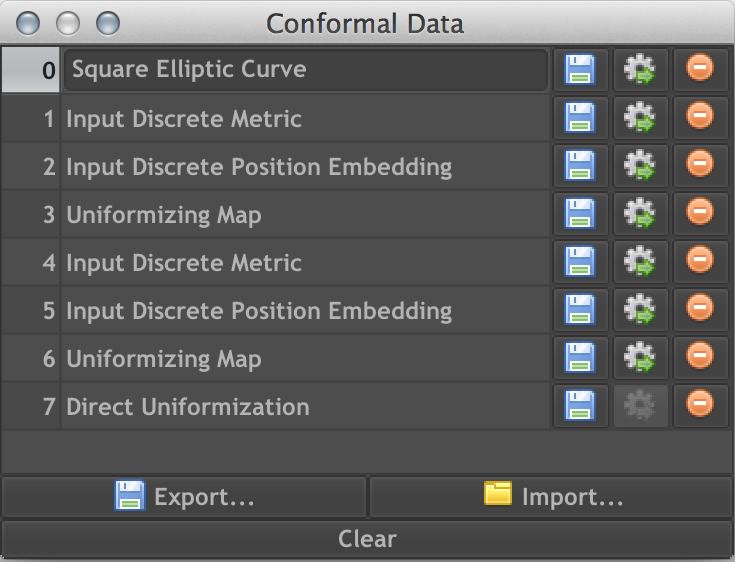
\includegraphics[width=\linewidth]{conformllab/conformal_data.png}
\caption{XML data import and export interface of {\sc ConformalLab}.}
\label{fig:conformal_data}
\end{wrapfigure}
The data import and export panel, see Figure~\ref{fig:conformal_data},
provides functions to import and export data as described in Section~\ref{sec:conformal_data}.
Data can be loaded into memory via the Import button. A table lists the entries of the loaded file.
Loadable are {\tt ConformalDataList} as well as single data instances. The entries of a
{\tt ConformalDataList} are listed in the table of the panel. Each of the rows contains buttons
to save the data to disk (blue disk), load it into the program (gear with green arrow), or delete 
it from the list (red circle).
The function of the load button depends on the data type. A {\tt HalfedgeEmbedding} is
loaded as geometry. A {\tt HalfedgeMap} defines geometry together with texture coordinates
and boundary identifications. If suitable boundary identification is given a uniformizing
group is calculated and visualized.

\begin{wrapfigure}{R}{0.4\textwidth}
\centering
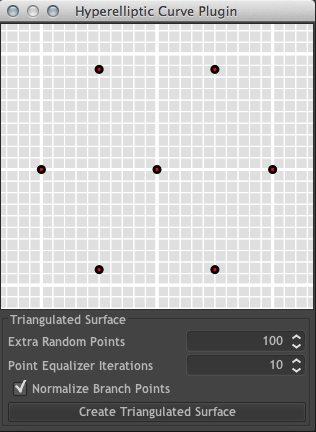
\includegraphics[width=\linewidth]{conformllab/hyperelliptic_curve.png}
\caption{Hyperelliptic curve interface of {\sc ConformalLab}.}
\label{fig:conformal_hyperelliptic}
\end{wrapfigure}

\begin{wrapfigure}{R}{0.4\textwidth}
\centering
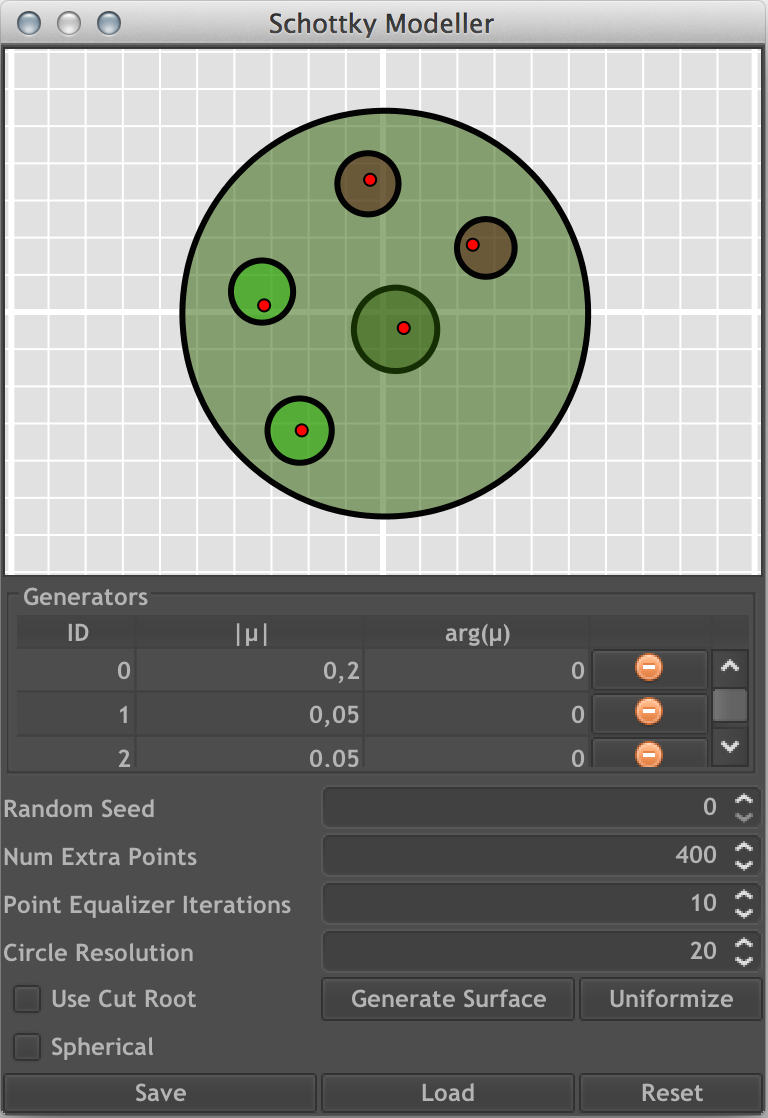
\includegraphics[width=\linewidth]{conformllab/schottky_modeller.png}
\caption{The Schottky modeller user interface of {\sc ConformalLab}.}
\label{fig:conformal_schottky}
\end{wrapfigure}

\begin{wrapfigure}{R}{0.3\textwidth}
\centering
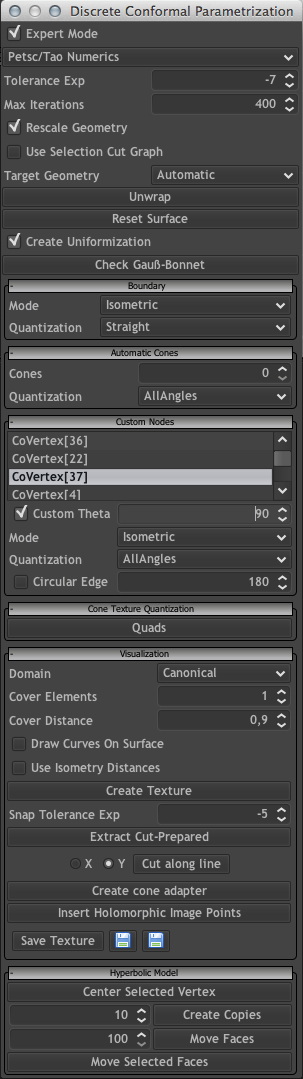
\includegraphics[width=\linewidth]{conformllab/main_interface.png}
\caption{The main interface of {\sc ConformalLab}.}
\label{fig:conformal_main}
\end{wrapfigure}



\subfilebibliography
\end{document}

%%% Local Variables:
%%% TeX-master: "Thesis.tex"
%%% End: